%----------------------- Research Proposal Master Document ------------------------
%
% Created by: Shane Reynolds 2020-02-29
%
%----------------------------------------------------------------------------------

%------------------------ Preamble and bibliography resources
\documentclass[12pt]{article}
%!TEX root = research_proposal.tex

\usepackage{geometry}
\geometry{a4paper,inner=3cm, outer=3cm, top=2cm, bottom=3cm}
  \pdfpagewidth=\paperwidth 
  \pdfpageheight=\paperheight
  % This acts as a failsafe to ensure things aren't stretched or moved when it's finally printed as a PDF.

\setlength{\parindent}{1em}  % Sets the length of the paragraph indent. Current setup has a an indent. Disable this if you activate the return line above.

% Double or one and a half spacing.
\usepackage{setspace}
  \onehalfspacing

\usepackage{booktabs}
% makes tables look sweet with top, mid, and bottom rules

\usepackage{graphicx}
  \DeclareGraphicsRule{.tif}{png}{.png}{`convert #1 `dirname #1`/`basename #1 .tif`.png}
% Graphics. Remove me and you won't have any figures, and that would be very boring.

\usepackage[usenames,dvipsnames,svgnames,table]{xcolor}
% Adds the ability to make coloured text and lines throughout the document. See documentation for xcolor.

%-------------------- Tables, figures and captions
\usepackage[font={small},labelfont={bf},margin=4ex]{caption}
% Makes bold labeled and smaller font captions. Must be loaded before the longtable package to avoid conflicts! 

\usepackage{longtable}
% Long tables (more than one page). Different headers and footers for beginning and end pages, etc.

\usepackage{afterpage}
% Make a longtable start on the next clear page, but fills the previous one with text first (no random gaps in the text-from long tables anymore! Man, the day I discovered this...)

\usepackage{booktabs}
% Nice looking tables and lines in tables

\usepackage{multirow}
% Entries in tables over multiple rows

\usepackage{lscape}
% Pages in landscape

\usepackage{wrapfig}
% Allows figures that don't take up the entire width of the page, wrapping the text around the figure

%-------------------- Special symbols and fonts
\usepackage{amssymb}
% Maths symbols

\usepackage{siunitx}
% important package for scientific papers

%-------------------- Document sections, headers, footers, and bibliography
\usepackage{fancyhdr}
% for creating different headers and footers
 
%-------------------- Graphics path specification
\graphicspath{{./fig/}}

%-------------------- Draft water mark
%\usepackage[hidelinks]{hyperref}		% for watermark
%\usepackage[printwatermark]{xwatermark}	% for watermark
%\usepackage{tikz}						% for watermark
%\usetikzlibrary{shapes,arrows}			% for watermark

%-------------------- Function to place draft watermark on document
%\newsavebox\mybox
%\savebox\mybox{\tikz[color=red,opacity=0.3]\node{DRAFT};}
%\newwatermark*[allpages,color=red!30,angle=45,scale=7,xpos=-20,ypos=20]{\usebox\mybox}

%-------------------- Bibliography
\usepackage[backend=biber,style=ieee]{biblatex}
% This is the package that lets you create a bibliography. I recommend reading the biblatex documentation to understand all the options i've specified here. BibLaTeX was created to replace BibTeX. It has lots of extra fields and options. I'm also using the biber backend here rather than the default, it copes with unicode and so can deal with accented characters easily.

% Currently this is set up to use RSC style references with article titles displayed. You can change this to another numeric style, there are other numeric styles available: Vancouver, american chemical society, american institute of physics, etc. As well, there are author-date styles available. Most journals or styles you can think of are available and you're not restricted to use any particular referencing style at CDU. Royal society of Chemistry is just what I use. I'd recommend you talk to your supervisor about what referencing style to use, usually one that is common in your chosen field.

% Traditionally you would use BibTeX, a special build of TeX, for your bibliogrpahy.The newer biblatex package is a more powerful bibliograpy management tool for LaTeX. You can make multiple, chapter based bibliographies, footnote bibliographes, sort your references by date, author, order cited, essentially by any bit of citation data you happen to have. You can also have a seperate library with a differnet format for say books and articles. Or if you're a PhD student, the thesis references and your a list of YOUR publications. That siad. If you want to use the old way this is it below.

%-------------------- Hyperlinks in your document.
\usepackage[unicode=true,colorlinks=true,linkcolor=black,citecolor=black,urlcolor=black,breaklinks=true]{hyperref}
% The hyperref package allows you to have clickable links in your pdf. It also allows you to have the mailto link associated with your name. It can be  a bit finicky, so load it last.

%\usepackage[hyphens]{url}
% package used to properly specify

%-------------------- Command renewals, New commands etc.
\renewcommand{\thefootnote}{\alph{footnote}}              
%letters for footnotes instead of numbers to avoid confusion with references.

%-------------------- Function to create a small title block
\newcommand{\namelistlabel}[1]{\mbox{#1}\hfil}
\newenvironment{namelist}[1]{%1
\begin{list}{}
    {
        \let\makelabel\namelistlabel
        \settowidth{\labelwidth}{#1}
        \setlength{\leftmargin}{1.1\labelwidth}
    }
  }{%1
\end{list}}

 % this must be left as \input, \include wont work in the preamble
\usepackage{mathptmx}

% This is where you load your bibliography file. If you use change to BibTeX and natbib in the pramble comment it out.
\addbibresource{../zz_administration/00_bibliography_db/bibliography_db.bib}

%-------------- Information For The Title Page
\title{ENG720: Research Proposal}
\author{}
\date{}

%------------------------ Main Document --------------------------
\begin{document}
	\maketitle

	\begin{namelist}{xxxxxxxxxxxx}
		\item[{\bf Title:}]
			Automatic generation control of a two area power system using deep reinforcement learning
		\item[{\bf Author:}]
			Shane Reynolds
		\item[{\bf Supervisor:}]
			Charles Yeo \& Stefanija Klaric
		\item[{\bf Degree:}]
			Bachelor of Engineering (Honours)
	\end{namelist}

%-------------- Table of contents
	\phantomsection \pdfbookmark[0]{Contents}{Contents}
	{\small\tableofcontents}
	\newpage

%-------------- Sections
	\section{Introduction \& Background}
In 2018, approximately 261$\si{\tera\watt\hour}$ of power was generated in the Australian electricity sector. Renewables contributed 19\% of the total generation, an increase from 15\% in 2017. The Department of Industry, Science, Energy and Resources have observed an increase in renewable energy generation year-on-year in the electricity generation market since 2008, as shown in Figure \ref{fig:energyts} \cite{Diser2020}.
\begin{figure}[ht]
	\centering
	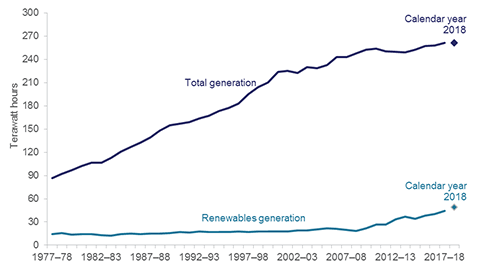
\includegraphics[height=7cm]{australian_generation_profile}
	\caption{Power generation from renewable sources (light blue line), and total power generation (dark blue line) in Australia from 1977 to 2018.}
	\label{fig:energyts}
\end{figure}

One of the benefits of transitioning from thermal sources of power generation to renewable sources is reduced greenhouse gas emissions \cite{IPCC2012}; however, this transition is not without its drawbacks. With an increased reliance on renewable power generation sources posing challenges for power system stability owing to load management. A recent example is the system failure in Alice Springs, caused by an event cascade that was triggered by cloud cover shadowing a solar array. The system failure left residents in Alice Springs without power for approximately eight hours \cite{UCNT2019}. An independent investigation highlighted that poor control policies were one of the factors that contributed to the blackout. In this instance, the generator provisioned to ramp up in the event of cloud cover was unable to be controlled. Moreover, generators that were still under the control regime were issued operating set points above their rated capacity, that resulted in thermal overload and subsequent tripping from the protection system \cite{Wilkey2019}.

Current control methods use classical feedback loop techniques. These methods can be brittle when faced with system changes, or scenarios which they were not designed for. An improved controller would be one that can learn and adapt its controller to an unseen system or event, given some broad control objective. This research proposes a deep reinforcement learning (DRL) agent for controlling the frequency of a power system consisting of multiple generators, and multiple load demands with individual stochastic profiles.

\subsection{Power Systems and Frequency}
Interconnected power systems are comprised of power generating units and energy storage systems connected to transmission and distribution networks. Generated power is used to service load demand. A single line diagram of a power network can be seen in Figure \ref{fig:generation}. The left hand side of the diagram shows thermal generation units, such as coal and nuclear, in addition to renewable sources of generation, like wind and solar. The right hand side of the figure shows the distribution network and the consumers of generated energy: industry and households.
\begin{figure}[ht]
	\centering
	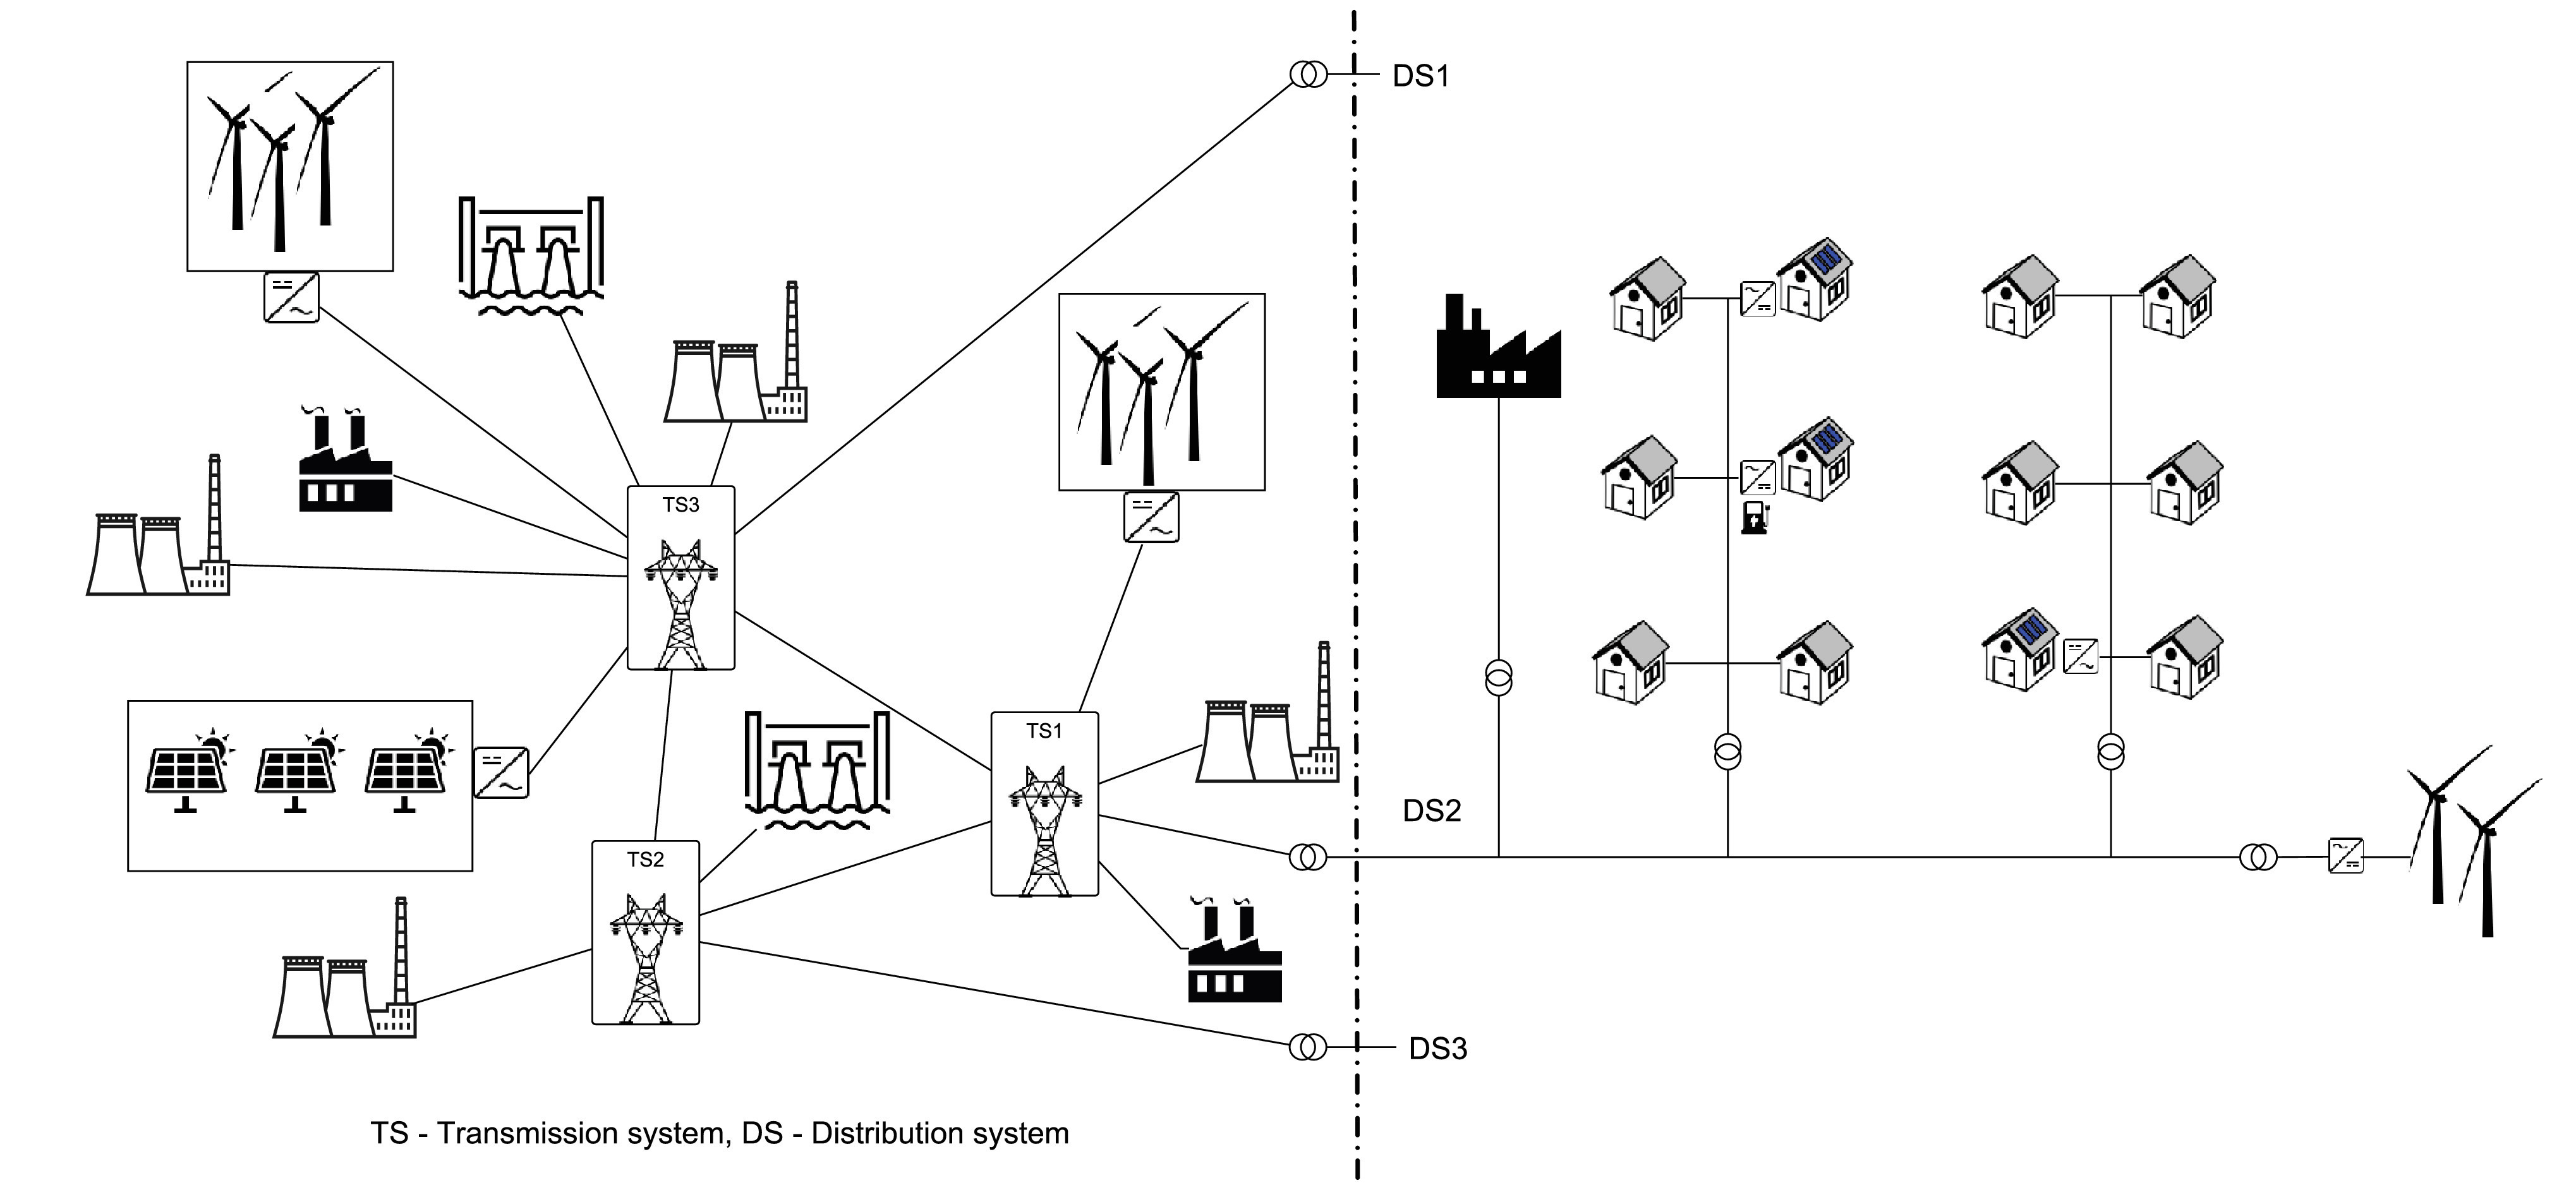
\includegraphics[scale=0.85]{power_system}
	\caption{A single line diagram of a typical power system taken from \cite{Glavic2019}. The image shows points of generation from thermal and renewable sources, and the subsequent supply of generated energy to meet load demand through the transmission and distribution network.}
	\label{fig:generation}
\end{figure}

One of the key elements to successful operation of interconnected power systems is ensuring total load demand is matched with total generation while taking into account power losses involved with generation, transmission, and distribution \cite{Wood2013}. To understand why it is important to match generation with load demand it is useful to first consider the basic operation of a single thermal generator. 
\begin{figure}[h]
\centering
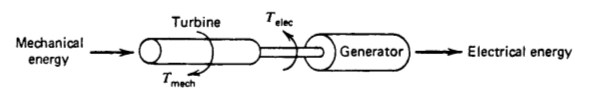
\includegraphics[height=1.4cm]{generation}
\caption{A thermal generation unit consists of a prime mover (turbine), and a synchronous machine. This image was taken from \cite{Wood2013}.}
\label{fig:turbine}
\end{figure}

The essential elements of a thermal generator are a prime mover (such as a gas turbine) and a synchronous machine, as depicted in Figure \ref{fig:turbine}. The prime mover provides mechanical torque, $T_{mech}$, which drives the synchronous machine producing electrical energy. In response, the synchronous machine creates an opposing torque which depends on the size of the load demand from households and industry. This opposing torque is referred to as electrical torque and is denoted as $T_{elec}$. If $\alpha$ represents angular acceleration of the generator rotating mass, and $I$ is its moment of inertia, then by Newton's second law:
\begin{equation}
\sum T_i = I \alpha \label{eq:1}
\end{equation}

Equation \ref{eq:1} shows that when $T_{mech}$ equals $T_{elec}$ the system will be in a steady state of zero angular acceleration with a constant angular velocity $\omega$. Now, if $T_{mech} > T_{elec}$, then the system has some angular acceleration causing the angular velocity $\omega$ to increase. This results in a frequency increase in the system. Conversely, if $T_{mech} < T_{elec}$ then the angular velocity $\omega$ will decrease, resulting in a frequency decrease. What makes this situation interesting is that, at any point in time, the total electrical load demand will fluctuate stochastically as businesses and households switch grid connected devices or motors on and off. The implication is that an uncontrolled system will have a continually changing frequency. Australia's electricity network is designed to operate at a frequency of 50$\si{\hertz}$. In the majority of network scenarios the Australian Energy Market Operator (AEMO) has a desired operating range for frequency which lies between 49.85$\si{\hertz}$ and 50.15$\si{\hertz}$ \cite{AEMOfreqdev}. Similarly, the Power and Water Corporation (PWC) Network Technical Code for the Northern Territory states that under normal operating conditions frequency should be maintained in the range 49.80$\si{\hertz}$ to 50.20$\si{\hertz}$ \cite{Pwc2013}. Operation outside of specified ranges can cause damage to electrical equipment such as transformers or motors, which are designed to operate at specific frequencies \cite{Sen2014}. Network designers engineer protection schemes so that sustained frequency excursions outside of the allowed range will cause equipment to trip from the network \cite{AEMOpowerfreqriskrev}.

\begin{figure}[ht]
	\centering
	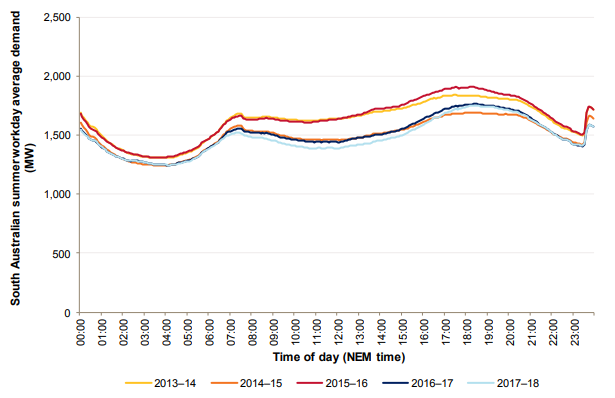
\includegraphics[height=7cm]{load_profile}
	\caption{Intraday timeseries of weekday energy demand profile in South Australia during summer \cite{Aemosaenergyrep}.}
	\label{fig:energydemand}
\end{figure}

\newpage

Protection schemes tripping equipment from the network is undesirable since this can leave households and industry without power, resulting in economic loss. Further, if disconnections are uncontrolled then this can reduce system stability further \cite{AEMOpowerfreqriskrev}. System controllers, such as the AEMO and PWC, are therefore interested in being able to control the system to follow changes in load demand so that system frequency is maintained in the allowable range. Additionally, they are interested in control mechanisms to restore frequency excursions as a result of unexpected disturbances. System controllers can use historical data, like that shown in Figure \ref{fig:energydemand}, to forecast daily demand profiles with some reliability. This type of forecasting does not help when trying to predict the occurrence of random disturbances, however, it does provide a starting point for estimating required generation needed to meet demand. It is important to note that forecasting is not perfect. Inevitably mismatches in supply and demand will occur causing small imbalances between $T_{mech}$ and $T_{elec}$, resulting in a change to angular velocity $\omega$ and the network frequency \cite{Glover2012}. To perfectly match supply and demand, system controllers use generators referred to as regulating units \cite{Kothari2011}. A regulating unit is a generator that has capacity to increase or decrease mechanical torque $T_{mech}$. If the system controller has a sufficient number of regulating units it can perform two functions: load following; and restoring the system to stable operating conditions in the event of a disturbance \cite{Grainger1994}. Using a regulating unit to load follow is referred to as the provision load following ancillary services \cite{AEMOancilliaryserv}. Load following control adjusts regulating units slightly to match supply perfectly with a demand load profile, like that shown in Figure \ref{fig:energydemand}. Using a regulator to restore the system after a disturbance is referred to as providing spinning reserves \cite{AEMOancilliaryserv}.

\begin{figure}[ht]
\centering
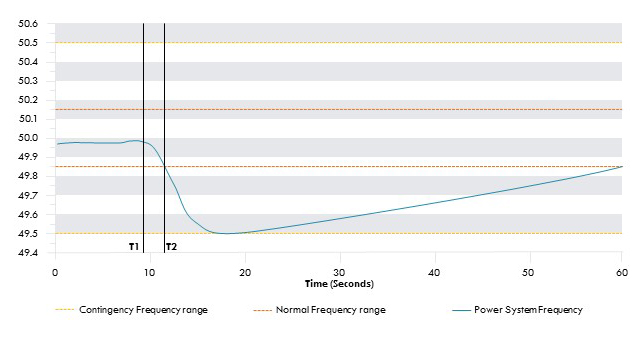
\includegraphics[height=8cm]{frequency_arrest}
\caption{A frequency disturbance occurs just before the 10 second mark, and regulating units ramp up their generation to first arrest the disturbance, and provide the subsequent correction, returning system frequency to 50$\si{\hertz}$.}
\label{fig:freqarrest}
\end{figure}

When used in this fashion it is important to note that the regulating unit is not responsible for arresting frequency excursions, rather, it is used to restore the system back to the allowable frequency operating range after the frequency excursion has been arrested. An example of a frequency excursion, arrest, and subsequent restoration can be seen in Figure \ref{fig:freqarrest}. AEMO and PWC do not require all generators on the network to act as regulating units since adequate frequency control can be achieved using a subset of the total available generators.

\subsection{Frequency control for a single area system}\label{oneareapowersystem}
The power system model shown in Figure \ref{fig:energyts} depicts total generation coming from many generation assets - this is complex to model. Researchers often find it useful to divide generation assets into sub-groups referred to as control areas \cite{Kothari2011}. A control area is defined as a subset of generators which are in close proximity to each other and constitute a coherent group that speed up and slow down together, maintaining their relative power angles \cite{Kothari2011}. The total network is therefore comprised of many interconnected control areas. An example of a series of interconnected control areas can be seen in Figure \ref{fig:interconnectedpa}. Notice that for each area there is only one load and one generator. Typically, for each control area, researchers will aggregate many loads into a single load, and many generators into a single generator. This simplifies the model further \cite{Grainger1994}.
\begin{figure}[ht]
	\centering
	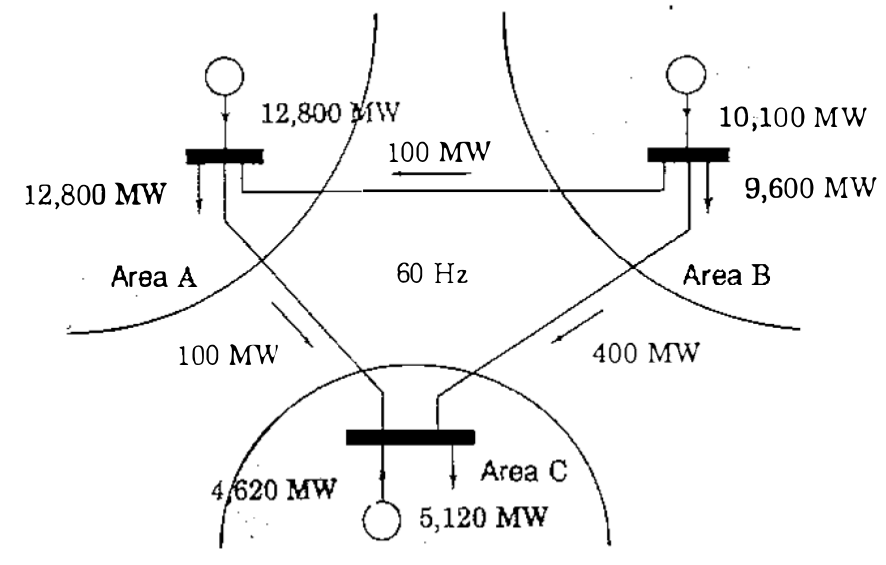
\includegraphics[height=8cm]{multiple_area_system}
	\caption{An example of three interconnected control areas in a 60$\si{\hertz}$ power system. The interconnections allow power to flow from one area to another, allowing generators to service loads from different areas. Each control area is consists of many generators and loads, but are modelled with a single generator and single load, respectively \cite{Grainger1994}.}
	\label{fig:interconnectedpa}
\end{figure}

The simplest power system to control is one that consists of a single control area. A single control area power system has no interconnections to any other control area. It is comprised of consumer load demand, and a set of generators, some of which are acting as regulating units. As previously mentioned, for modelling simplicity, loads are aggregated to a single load, and generators are aggregated to a single generator. This simple system is a classic example and well understood. It is generally acknowledged that a governor feedback control regime can successfully perform frequency control of a single area power system \cite{Wood2013, Grainger1994, Kothari2011}. Most introductory textbooks on power systems cover governor control of this system. A particularly well laid out approach to developing linear models for the turbine, generator load, and governor can be found in \cite{Kothari2011} - the full model is shown in Figure \ref{fig:singleareacontrol}. The leftmost block is a first-order linear model of the speed governor, the second block is a first-order model of the turbine, which the controller directly acts on. The final block is the generator load, which is also a first order system. The over all system model is a second order linear model, with a first order controller.

\begin{figure}[ht]
\centering
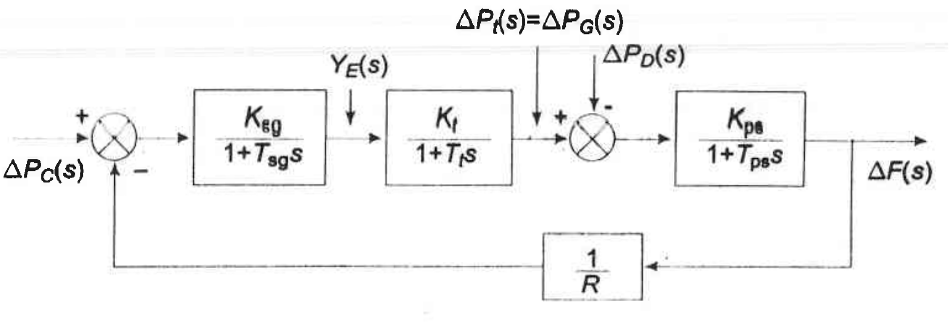
\includegraphics[height=5cm]{single_area_control}
\caption{A classical feed back control approach to a second order linear system. The second order system is comprised of a first order model for both the turbine, and generator load. The controller is modelled as a first order system \cite{Kothari2011}.}
\label{fig:singleareacontrol}
\end{figure}


\subsection{Frequency control for two area system}
The single area system presented in Section \ref{oneareapowersystem} is useful to help understand the role of governors in controlling power system frequency, however, a single area model is too simple. In reality, power systems are comprised of many control areas connected by transmission lines (referred to in the literature as tie lines). Often it is the case that there is some net power transfer over the tie lines, enforceable by contract.

\begin{figure}[ht]
	\centering
	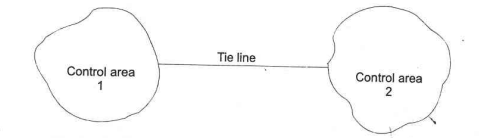
\includegraphics[height=3cm]{two_area_system}
	\caption{Two area power system is comprised of generators and load connected via a tie line. Power flows from one area to the other depending on economic contracts.}
	\label{fig:twoareapower}
\end{figure}

Distinct control areas are typically thought of as different participants in the generation market, or simply as different regions in which generation assets are based \cite{Kothari2011}. The simplest model which includes tie lines is the two area power system, shown in Figure \ref{fig:twoareapower}. The control objective with this system is to maintain the inter-area power transfer, whilst regulating the frequency of each area. Simply relying on governor control in each area will not satisfy the control objective. To see this, consider control area A supplying a 50MW load, with a contract to supply control area B with 20MW over the tie line connecting them. If control area B also has a 50MW load, then it is supplying only 30MW to satisfy the demand in this area. Now suppose a 30MW load increase was observed in the demand for area A. Relying on governor control will see generators from both area A and area B speed up in response to this increased load. Ultimately the increased power demands will be met, however, the power transfer over the tie line is likely to be less than the contracted 20MW value, which is problematic. Contract violations due to system instability and control issues do not allow for a stable market in which energy can be reliably traded. Fortunately, two area power systems are well understood. Linear models have been developed to simulate these systems, and classical control approaches have been successfully implemented to meet the new control objectives. In order to achieve this, a metric called Area Control Error (ACE) is used. This measures the distance from a target frequency as well as the deviation from tie-line contractual obligations. The implementation of this control system is shown in Figure \ref{fig:twoareacontrolblock}.

\vspace{2cm}

\begin{figure}[ht]
	\centering
	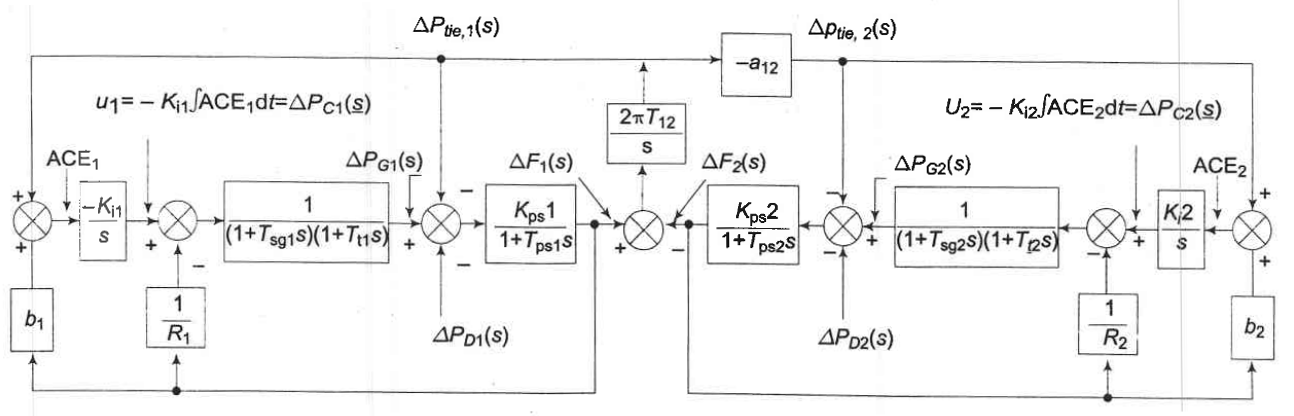
\includegraphics[height=4.8cm]{two_area_control_block}
	\caption{A classical feed back control approach to a two power area system. Image taken from \cite{Kothari2011}.}
	\label{fig:twoareacontrolblock}
\end{figure}

\newpage

\subsection{Reinforcement learning}
Reinforcement Learning (RL) is a branch of machine learning that is concerned with how agents make sequential decisions to maximise some notion of a cumulative reward. It is a simple idea that allowed Google's Deep Mind to beat the worlds best players in the game of Go \cite{Silver2016}. One of the important aspects of RL is the underlying architecture of the model allows for generalisation to many different applications, albeit the models do require training with different data sets for each application. Subsections 1.4.1 and 1.4.2 provide a brief overview of key architectural components of RL, and subsection 1.4.3 gives details on how these components are implemented to build an agent that can perform a control activity for some application.

\subsubsection{Markov decision process}
Suppose an agent exists in some environment which is comprised of many discrete states, $s \in S$, such that $S$ denotes the state space. At any discrete point in time the agent can take an action $a \in A$, where $A$ denotes the action space. When the agent takes an action in a given state, the agent receives some reward, denoted with $r \in R$, where $R$ is the reward set. If an agent is in a given state, $s$, and takes and action, $a$, this will transition the agent to a new state, $s'$, and yield reward, $r$, with some given probability - these are referred to as state transition probabilities. Transition probabilities are denoted as follows:
\begin{equation}
P(S_{t+1}=s', R_{t+1}=r \ | \ S_t = s, A_t = a)\label{eq:2}
\end{equation}

The set of parameters, outlined above, make up a framework referred to as a Markov Decision Process (MDP) \cite{Bellm1957}. The MDP framework is important to understanding how RL works, however, it must be noted that it is not necessary for the agent to have any information about the state transition dynamics to develop an effective control regime.

\subsubsection{Return, episodes, and policy}
As the robotic agent takes actions at each discrete time step, it receives a reward. The cumulative sum of this reward is referred to as the return \cite{openai2018}. The return is denoted, for $N$ discrete time steps, as:
\begin{equation}
G_t = r_t + r_{1+1} + r_{t+2} + \ldots + r_{N-1}\label{eq:3}
\end{equation}

Often it is convenient to make future rewards less important than more immediate rewards. This is achieved by multiplying each reward in the sequence by a discount factor, $\gamma \in [0,1]$. Equation \ref{eq:3} then becomes:
\begin{equation}
G_t = r_t + \gamma \ r_{1+1} + \gamma\mystrut^2 r_{t+2} + \ldots + \gamma\mystrut^{N-1} r_{N-1} = \sum_{k = 0}^{N-1} \gamma\mystrut^k r_{t+k}
\end{equation}

The duration of time that an agent will cumulate reward is referred to as an episode. An episode is made up of a beginning, middle, and an end. Typically this consists of an RL agent beginning in some initial state. As time passes the agent takes actions, undergoes state transitions, and collects rewards. The episode concludes when the agent reaches a terminal state. At the episode conclusion, the agent receives it's cumulative reward \cite{Kaelbling1996}.

Finally, in order for the robot to act within the environment, it needs to have a policy. A policy, $\pi$, is defined as a mapping from states to actions, that is, a rule which determines what action the robot will take for a given state. A deterministic policy, $\pi (s)$, maps a single action to a single state. A stochastic policy, $\pi (a | s)$, defines a probability distribution over the actions for a given state. An optimal policy, denoted $\pi^*$, is a policy which will maximise the cumulative reward that the agent receives over an episode \cite{Bellm1954}. It can be thought of as the best control policy an agent can have for the given the environment and cumulative reward function.

\subsubsection{How does an RL agent learn?}
The main objective of RL is to develop an optimal policy. There are many algorithmic approaches to building an optimal policy. One of the most common implementations is called Q-Learning. This approach focuses on finding q-values for each state-action pair. A q-value can be thought of as an ordinal value that is discovered and assigned to a state-action pair which tells the agent how important an action is relative to the rest of the actions in a given state. To discover q-values, the agent normally starts with a randomised policy meaning that all the q-values are set to zero. This will lead the agent to take actions at random to explore the state-action space. Higher q-values are assigned to state-action pairs that the agent determines are useful for building a high cumulative reward. Similarly, the agent assigns low q-values to state-action pairs which do not lead to high cumulative rewards. This process is akin to the agent modifying its policy. The q-value modification process is repeated for many episodes and eventually the agent policy converges on an optimal policy. Often the q-values are presented in a tabular format that the literature refers to as a Q-table. An example of a Q-table can be seen in Figure \ref{fig:qtable}. Rows represent different states, and columns represent different actions. Values in each cell provide an ordinance on how valuable each action is for a given state. The agent only needs to understand inputs that uniquely define a state, and the actions it can take in order to learn an optimal policy. It is not necessary for the agent to know the state transition dynamics of the system, described by Equation \ref{eq:2}. More concretely, an agent can learn to control a system for which is does not have a mathematical model.
\begin{figure}[ht]
	\centering
	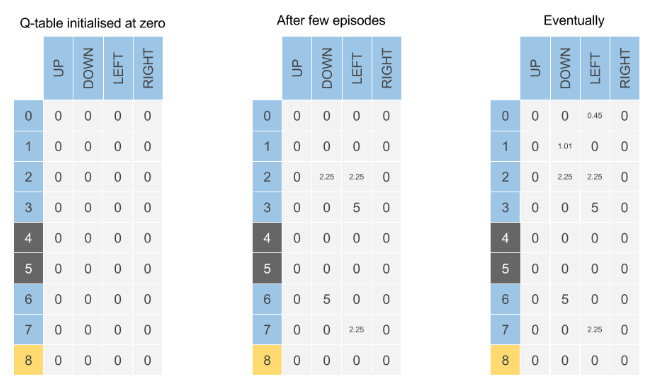
\includegraphics[height=8cm]{q_table}
	\caption{The Q-table on the left shows the initialised policy when the agent begins learning. The middle and rightmost Q-tables show the agent developing an understanding of which actions are valuable in which states.(REFERENCE)}
	\label{fig:qtable}
\end{figure}

\subsection{Deep reinforcement learning}
For low dimensional state-action spaces RL leads to policy convergence in a reasonable time frame. As state-action space dimensionality increases models like Q-Learning experience difficulty. The main reason for this is that it becomes difficult for the discrete RL algorithm to visit every state-action pair unless the computational power is dramatically increased. Researchers often refer to this as the curse of dimensionality. Stopping policy discovery early for problems with high dimensionality results in Q-tables that are sparse (mostly populated with zeros).
\begin{figure}[ht]
\centering
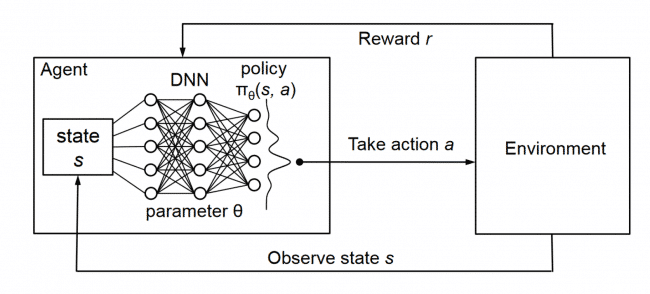
\includegraphics[height=5cm]{deep_reinforcement_learning}
\caption{The agent interacts with the environment by taking actions, which affect the state it is in and the reward it receives. The rewards allow agent to adjust the weights in the neural net to build better policies.}
\end{figure}

The interpretation is that the agent does not have complete knowledge of optimal actions for every given state, leading to the derivation of sub-optimal policies. To get around this problem, for RL problems with high dimensional state spaces, the discrete Q-table is replaced with a function approximator known as a neural network. A high level overview of the architecture can be seen in Figure 11. It is the neural network architecture in which the agent policy is implemented. As the agent learns, it adjusts weights in the neural network to change the policy. This is approach is powerful because neural networks are good at generalising, and hence the agent does not need to visit every state action pair to be able to make good decisions.
	\section{Research Aims}
The principle aim of this research is to compare the performance of classical engineering control methodologies against a control system based on a DRL agent, when tasked with performing AGC for load following tasks on a two area power system. The ultimate research outcome will be to provide comment on the feasibility of using DRL agents for this purpose.
	\section{Scope}
The proposed research is only concerned with the task of load following using DRL and classical control agents. Load following is defined as maintaining system frequency within PWC's allowable region of 49.80$\si{\hertz}$ to 50.20$\si{\hertz}$ for normal operating conditions. Task involving frequency restoration following a disturbance event may be considered, time permitting. The key performance aspects that will assessed, for DRL and classical, are the controller's ability to:
\begin{itemize}
	\item maintain system frequency to the desired nominal 50$\si{\hertz}$ value;
	\item maintain the tie line power flow between control areas at the scheduled value.
\end{itemize}

The research will not consider power systems larger than a two area power system. Each power area will consist of one regulating generator, and one stochastically fluctuating demand profile. The research will not consider the control of system variables other than frequency, however, note that other system variables may be used as input features under agent training and inference regimes. Comparison of DRL agent performance will be made against theoretical models of classical control architectures. Performance against practical control architectures implemented by PWC (or other utilities) will not be considered. Research will be conducted in an entirely simulated environment. Agent performance on real hardware will not be explored.
	\section{Approach}

\subsection{Required data sources and data management}\label{datamanagement}
Training a DRL agent to change regulating generator set points in order to maintain system frequency and tie line requirements while load following will require realistic demand profiles. Similarly, performing system restoration after a disturbance will require realistic disturbance scenarios. Ideally this data would come from a major utility provider, such as PWC, in the form of a time series dataset with a large number of features, and high sample rate. To this end, data acquisition will be one of the principle objectives in the early stages of research. Should the acquisition of data from PWC or TGEN be viable, a data management plan will need to be developed which addresses concerns around the sensitivity and security of the data. The data management plan will outline where data the will be stored, and how the data will be treated (or disposed of) once the research is concluded.

In the event data cannot be acquired from a utility provider, a simulated data set may need to be used. This would be achieved by understanding key statistical parameters of a typical load demand profile, and using these to create a process which emulates the load demand signal. This could also be done for other system variables; however, care would need to be taken ensuring correlations are preserved between multiple variables in the simulated time series dataset.

\subsection{Theoretical approach}
In order to establish the most effective way to approach this research problem, a clear understanding of the benefits and limitations of existing AGC approaches is needed. Determining justifications for practical AGC design choices will help to uncover important performance aspects the research should focus on. Equally important is exploring alternative approaches to AGC that researchers have investigated historically. This should have a particular focus on the use of Neural Networks and DRL agents for AGC. A literature review will be the main avenue for achieving this.

As discussed in \S{}\ref{datamanagement}, securing load demand profile datasets from a major utility provider, or developing simulated load profile datasets based on local load profile characteristics is an important aspect of this research and is a priority. Similarly, investigating suitable software packages to develop the power system simulation model, and investigating suitable programming languages to implement a DRL agent are necessary. Exploring the field literature and finding published examples will be a key stepping stone. It will be important to understand how other researchers integrated the DRL agent with the simulation environment.

A simulated model of the two area power system will be developed. The decision to use a linear or non-linear model will be informed by the literature review. It may be interesting to explore DRL agent performance on both linear and non-linear models since one of their advantages is that they have a demonstrated capacity for controlling non-linear systems. Classical engineering system modelling techniques will be employed for power system model development \cite{Ogat2010}. An area of interest is how sensitive a DRL agent control regime is to changes in key plant parameters --- for a given set of parameter changes both DRL agent and classical control architecture performance could be compared to see which controller is more brittle.

A feedback loop controller will be developed for the two area power system using models presented in the literature. A DRL agent will be developed using an architecture that takes continuous input signals and provides continuous output signals. There are a number of established DRL models presented in texts like Sutton and Barto that will be explored to determine the most ideal approach \cite{Sutton2018}. Time permitting, a DRL model that uses discrete input and output signals will be developed. Discrete models offer lower performance due to errors introduced in the discretisation process, but can be computationally less expensive than continuous models. DRL models will be trained using data previously acquired either from a utility provider, or from simulation. Metrics will be selected to measure the performance of both controllers. Choice of metrics will be informed by earlier research (mentioned above). Control models differences in performance will be compared --- this will be one of the major focuses of the research.

The full list of tasks for the research design are as follows:
\begin{enumerate}
	\item Enquire with power utility provider to secure data.
	\item Investigate ways to simulate data.
	\item Develop data management plan.
	\item Literature review centred on three central themes:
	\begin{enumerate}
		\item AGC
		\item DRL
		\item Applications of DRL to AGC.
	\end{enumerate}
	\item Investigate suitable software package to conduct simulation.
	\item Investigate suitable programming language to implement DRL agent and integrate with simulation.
	\item Develop and test simulation of two area power system.
	\item Develop feedback loop controller for two area power system.
	\item Test classical controller.
	\item Develop DRL model.
	\item Train and test DRL model.
	\item Execute control trials on both models for an unseen sequences of load demand data.
	\item Compare controller performance on AGC task.
\end{enumerate}

It is anticipated that there may be some issues in carrying out the aforementioned research design. The biggest risk would be the inability to successfully build the control models for both the classical engineering controller, and the DRL controller. For the classical engineering controller, the issue would be the inability to find the appropriate parameter settings to deliver stable control. With the DRL controller, the problem is selection of an appropriately sized neural network, and training hyper-parameters.
	\section{Deliverables Specification}
The main outcomes from this research is a conclusion about the feasibility of using DRL agents to provide AGC for a two area power system. The expectation is that the DRL agent will perform at least as well as a classical control approach. This expectation is based on the existing research in this field, which has shown that standard RL agents can perform AGC at least as well as classical control methods \cite{Ahamed2002}. If the research meets expectations, it should provide a pathway for the investigation of novel DRL models that could improve power system control. The ultimate goal would be to have a DRL agent that is always learning, so that it can adapt control strategies to unseen system conditions providing a more flexible and less brittle controller. This would help to avoid problems like that seen in the Alice Springs system blackout event.

A schedule of actual physical deliverable items can be found in Table \ref{tab:deliverables}, in chronological order.

\begin{table}[h]
	\centering
	\caption{A table of deliverable items and their respective due dates}
	\begin{tabular}{ll}
		\toprule
		Deliverable Item 						  & Due Date \\
		\midrule
		Online Topic and Supervisor Questionnaire & 05/03/20 \\
		Week 1 Progress report					  & 06/03/20 \\
		Research Plan 							  & 13/03/20\\
		Week 2 Progress report 					  & 13/03/20 \\
		Supervision Agreement Form 				  & 13/03/20 \\
		Literature Review 						  & 20/03/20 \\
		Week 3 Progress report 					  & 20/03/20 \\
		On-Line Library Skills Test				  & 20/03/20 \\
		Week 4 Progress report					  & 27/03/20 \\
		On-line Plagiarism Test					  & 27/03/20 \\
		Week 5 Progress report 					  & 03/04/20 \\
		On-line Ethics Test						  & 03/04/20 \\
		Technical Support and Funding Request 	  & 03/04/20 \\
		Week 6 Progress report 					  & 10/04/20 \\
		Reflective Progress Review Checklist 	  & 10/04/20 \\
		Week 7 Progress report 					  & 24/04/20 \\
		Draft Interim Report 					  & 29/04/20 \\
		Week 8 Progress report 					  & 01/05/20 \\
		Abstract 								  & 07/05/20 \\
		Week 9 Progress report 					  & 08/05/20 \\
		Submission of Ethics Form 				  & 08/05/20 \\
		Week 10 Progress report					  & 15/05/20 \\
		Poster 									  & 21/05/20 \\
		Week 11 Progress report					  & 22/05/20 \\
		Final Interim Report 					  & 28/05/20 \\
		Week 12 Progress report					  & 29/05/20 \\
		\bottomrule
	\end{tabular}
	\label{tab:deliverables}
\end{table}
	\newpage
	\section{Timeline}
\vspace{2cm}
\begin{figure}[ht]
	\centering
	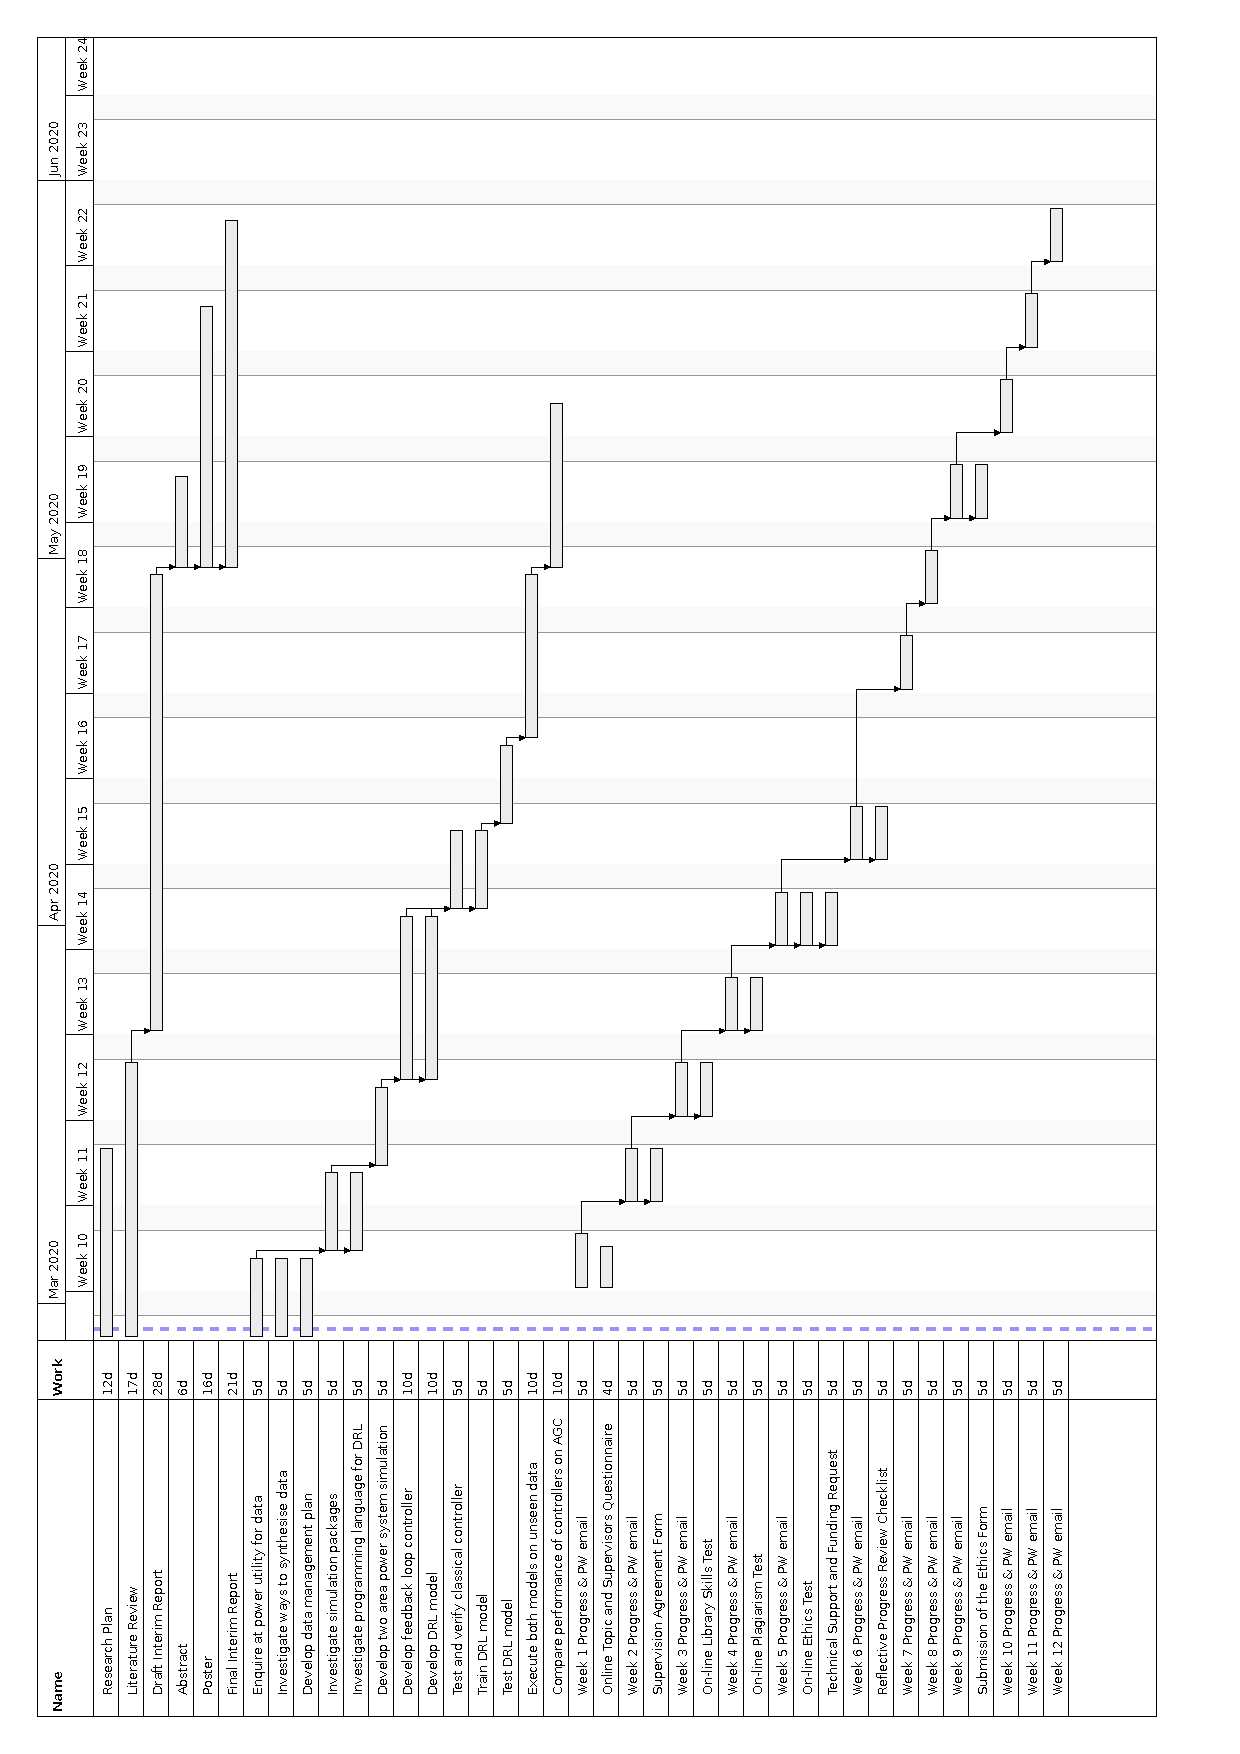
\includegraphics[scale=0.62]{../project_plan/project_plan}
\end{figure}
	\newpage
	\section{Resources}
In order to reach research objectives a computer with a Linux operating system featuring RAM, and a Graphics Processing Unit (GPU) will be required. The exact specifications of these computational resources are not yet known, and will be dependent on the size of the datasets, and the amount of computation required to train the DRL agent. Currently, access has been provided to an Intel Quad Core 3.2$\si{\giga\hertz}$ i5 CPU machine with 8GB of RAM, Nvidia GTX960 GPU, and Ubuntu operating system. It is expected these resources will be sufficient; however, in the event that greater computational power is needed, access to a virtualised environment, such as Amazon Web Services (AWS) set up to conduct DRL research, may be required. Using such a system can be expensive (1 hour of compute is approximately \$20AUD); however, AWS will often supply student research with a monetary credit. Approximately 10 hours of compute would be reasonably expected to achieve desired training outcomes for DRL agent. This allows for errors made in model training parameter specification, and subsequent retraining.
Table \ref{tab:resources} shows an itemised list of resources needed to complete this research, and their associate costs.

\begin{table}[h]
	\caption{Itemised list of resources needed to complete research and associated costs.}
	\centering
	\begin{tabular}{llr}
	\toprule
	Equipment 				& Details			 & Cost \\
	\midrule
	Intel Quad Core 3.2$\si{\giga\hertz}$ i5 CPU & pre-owned hardware 		& \$0 	 \\
	8GB of RAM 									 & pre-owned hardware		& \$0 	 \\
	Nvidia GTX960 GPU 							 & pre-owned hardware		& \$0 	 \\
	Ubuntu operating system 					 & open source software		& \$0 	 \\
	AWS GPU Large Instance 						 & ~\$20 @ 10 hours 		& ~\$200 \\
	Python 3.7 (Open AI Env)  					 & open source software 	& \$0 	 \\
	Matlab										 & CDU VM licence			& \$0 	 \\
	\midrule
	Total 										 & 							& \$200 \\
	\bottomrule
	\end{tabular}
	\label{tab:resources}
\end{table}

%-------------- Bibliography
    \cleardoublepage
    \phantomsection  \addcontentsline{toc}{section}{Bibliography}                    
    \printbibliography
    
    % Uncomment these two lines and remove the \printbibliography above and the \addbibresource{your_bibliography.bib} at the top of the document if you're using the BibTeX and natbib method to include you bibliography. For example, if you're using some online compiling systems which doesn't support biblatex. By default you shouldn't need to touch anything.
    %\bibliographystyle{plain}
    %\bibliography{your_bibliography}

\end{document}